%! Author = Stepan Oskin
%! Date = 2019-07-22

% Preamble
\documentclass[11pt]{article}
\usepackage{graphicx}
\usepackage{subcaption}

% Packages

% Document
\begin{document}

    \title{Relational databases \\
    Description of methodology \\
    Based on a course offered by DataCamp \\
    \textit{Introduction to Relational Databases}\cite{Grossenbacher2019} \\
    and other sources}

    \author{Stepan Oskin}

    \maketitle

    \begin{abstract}
        A relational database models real life entities, such as NHL players and NHL teams, by storing them in tables.
        The idea of a database is to push data into a certain structure \textemdash a pre-defined model \textemdash where you can enforce data types, relationships, and other rules.
        Each table must contain data from a single entity type.
        This reduces redundancy by storing entities only once.
        A database can then be used to model relationships between entities and to preserve data quality through such concepts as constraints, keys, and referential integrity.
        SQL, or Structured Query Language, can be used for querying, as well as building and maintaining databases.
    \end{abstract}

    \section{Relational Database} \label{sec:rdb}

    A relational database models real life entities, such as NHL players and NHL teams, by storing them in tables.
    Each table must contain data from a single entity type (\textit{e.g.}, NHL Players, NHL teams, \textit{etc.})
    This reduces redundancy by storing entities only once \textemdash for example, there only needs to be one row of data containing details of a certain NHL team.
    Lastly, a database can be used to model relationships between entities.
    For instance, an NHL player could have played for multiple NHL teams, while an NHL team includes many NHL players on their roster.

    An example of data organized with redundancy in attributes and without redundancy is presented in the two entity-relationship diagrams on figure~\ref{fig:ent_rel_diag}.
    The diagram on the left (fig.\ref{fig:with_redun}) models only one entity type \textemdash \texttt{university\_professors}.
    However, this table actually holds multiple entity types, and thus causes redundancy in entries, as the same professor and university can be present in multiple rows, for example, in cases where the professor is involved with multiple organizations within the same university.
    The updated entity-relationship model (fig.\ref{fig:without_redun}) would be better suited in this case.
    It represents three entity types \textemdash "professors", "universities", and "organizations" \textemdash in their own tables, with respective attributes.
    This reduces redundancy, as professors, unlike in fig.~\ref{fig:with_redun}, need to be stored only once.
    For each professor, the respective university is denoted through the \texttt{university\_shortname} attribute.

    \vspace{5mm}

    Characteristics of a relational database:
    \begin{itemize}
        \item real-life \textit{entities} become \textit{tables}
        \item reduced redundancy
        \item data integrity by \textit{relationships}
    \end{itemize}

    \begin{figure}[hbt!]
        \centering
        \begin{subfigure}[t]{.48\textwidth}
            \centering
            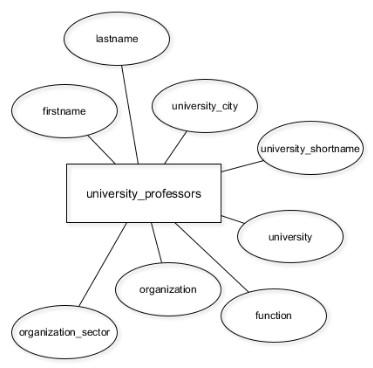
\includegraphics[width=\columnwidth,trim=4 4 4 4,clip]{img/ent_rel_diag1.png}
            \caption{with redundancy}
            \label{fig:with_redun}
        \end{subfigure}
        ~ %add desired spacing between images, e. g. ~, \quad, \qquad, \hfill etc.
        %(or a blank line to force the subfigure onto a new line)
        \begin{subfigure}[t]{.48\textwidth}
            \centering
            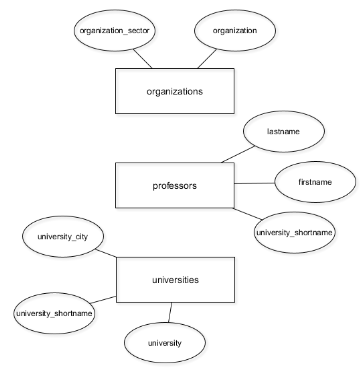
\includegraphics[width=\columnwidth,trim=4 4 4 4,clip]{img/ent_rel_diag2.png}
            \caption{without redundancy}
            \label{fig:without_redun}
        \end{subfigure}
        \caption{These two entity-relationship diagrams show examples of organizing data with redundancy in attributes (fig.~\ref{fig:with_redun}), and without redundancy (fig.~\ref{fig:without_redun}).
        Squares denote the so-called entity types, and circles connected to these denote attributes (or columns).}
        \label{fig:ent_rel_diag}
    \end{figure}


    \section{Integrity constraints} \label{sec:constraints}

    The idea of a database is to push data into a certain structure \textemdash a pre-defined model \textemdash where you can enforce data types, relationships, and other rules.
    Generally, these rules are called \textbf{integrity constraints}, although different names exist.

    \vspace{5mm}

    Integrity constraints can roughly be divided into 3 types:

    \begin{enumerate}
        \item \textbf{Attribute constraints}, \textit{e.g.}, data types on columns
        \item \textbf{Key constraints}, \textit{e.g.,} primary keys
        \item \textbf{Referential integrity constraints}, \textit{e.g.,} enforced through foreign keys
    \end{enumerate}

    Benefits of using constraints include:

    \begin{itemize}
        \item Constraints press data into a certain structure
        \item Constraints help with consistency, and thus data quality (\textit{e.g.,} by ensuring that the certain format is followed during manual or automated data entry)
        \item Data quality is a business advantage / data science prerequisite
        \item Enforcing constraints is difficult, but database management systems (\textit{e.g.,} PostgreSQL) help
    \end{itemize}

    \subsection{Attribute constraints} \label{subsec:att_constr}

    In its simplest form, attribute constraints are data types that can be specified for each column in a table.
    There are basic data types for numbers, such as \texttt{bigint}, or strings of characters, such as \texttt{character varying}.
    There are also more high-level data types, such as \texttt{cidr}, which can be used for IP addresses.
    Implementing such a data type on a column would disallow anything that doesn't fit the structure of an IP .

    Data types also restrict possible SQL operations on the stored data.
    For example, it is impossible to calculate a product from an \texttt{integer} and a \texttt{text} column.
    In case if a column with data type \texttt{text} contains numbers that need to be used in calculations, on-the-fly type conversions, or \textbf{type casts} can be used to allow the required operation using the \texttt{CAST} function in SQL .
    Examples of some data types from \textit{PostgreSQL documentation}\cite{ThePostgreSQLGlobalDevelopmentGroup2019} are presented on figure~\ref{fig:dtypes}.

    \begin{figure}[hbt!]
        \centering
        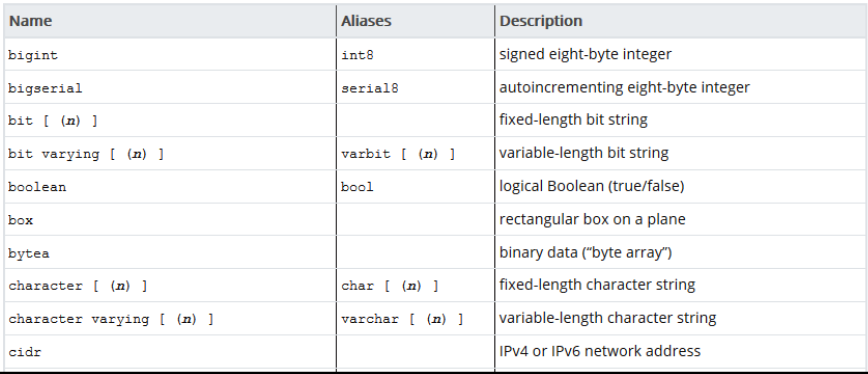
\includegraphics[width=1\linewidth,trim=1 1 1 1,clip]{img/dtypes.png}
        \caption{Beginning of the list of all data types from PostgreSQL documentation\cite{ThePostgreSQLGlobalDevelopmentGroup2019}.}
        \label{fig:dtypes}
    \end{figure}


    \section{\texttt{information\_schema} database} \label{sec:info_schema}

    SQL, or \textbf{Structured Query Language}, can be used for querying, as well as building and maintaining databases.

    \texttt{information\_schema} database is available by default in PostgreSQL and presents a \textit{meta database} that holds information about a relational database in PostgreSQL .
    \texttt{information\_schema} is not PostgreSQL specific, and is also available in other database management systems, such as MySQL or SQL Server.
    The \texttt{information\_schema} database holds various information in different tables, for example, in a \texttt{tables} or \texttt{columns} tables.

    \subsection{Querying \texttt{information\_schema} using \texttt{SELECT * FROM} syntax} \label{subsec:info_schema_q}

    \texttt{information\_schema} has multiple tables you can query with the known \texttt{SELECT * FROM} syntax:

    \begin{itemize}
        \item \texttt{tables}: information about all tables in your current database
        \item \texttt{columns}: information about all columns in all of the tables in your current database
        \item \ldots
    \end{itemize}

    \vspace{5mm}

    \textbf{Example}: get information on all table names in the current database, while limiting your query to the 'public' \texttt{table\_schema}.

    \vspace{5mm}

    \texttt{-- Query the right table in information\_schema \\
    SELECT table\_name \\
    FROM information\_schema.tables \\
    -- Specify the correct table\_schema value \\
    WHERE table\_schema = 'public';}

    \vspace{5mm}

    \textbf{Example}: get information on all column names in a particular table, while limiting your query to the 'public' \texttt{table\_schema}.

    \vspace{5mm}

    \texttt{-- Query the right table in information\_schema to get columns \\
    SELECT column\_name, data\_type \\
    FROM information\_schema.columns \\
    WHERE table\_name = 'nhl\_draft' AND table\_schema = 'public';}

    \medskip
    \bibliography{rdbms}
    \bibliographystyle{ieeetr}

\end{document}